\pdfminorversion=4
\documentclass[aspectratio=169]{beamer}
\usepackage{animate} % for animation
\usepackage{array,multirow,graphicx}
\usepackage{multicol}
\usepackage{etoolbox}
%\graphicspath{{/directory/to/image/folder/1/}
%              {/directory/to/image/folder/1/}}
\setbeamertemplate{caption}[numbered]
\setbeamertemplate{section in toc}[sections numbered]

% Hide subsubsections from TOC, but keep PDF bookmarks with beamer
\hypersetup{bookmarksopen=true,bookmarksopenlevel=4}
\setcounter{tocdepth}{4}

\renewcommand{\figurename}{Gambar.}
\renewcommand{\tablename}{Tabel.}

\usetheme[pageofpages=of,	% String used between the current page and the
							% total page count.
			alternativetitlepage=true,% Use the fancy title page.
			titleline=true,
			titlepagelogo=OK-LOGO-ITK.jpg
%          	 titlepagelogo=fig/jaist_logo.png
			]{Torino}
			% change /beamerinnerthemefancy.sty to resize the logo
\usecolortheme{freewilly}

\makeatletter
\patchcmd{\beamer@sectionintoc}{\vskip1.5em}{\vskip0em}{}{}
\makeatother

\author{Mifta Nur Farid \\
	miftanurfarid@lecturer.itk.ac.id}
\title{Komunikasi Data}
\subtitle{Pembahasan Kuis 2}
\institute{Teknik Elektro \\ Institut Teknologi Kalimantan \\ Balikpapan, Indonesia}
\date{\tiny Mei 17, 2021}

% The log drawn in the upper right corner.
\logo{
\includegraphics[height=0.13\paperheight]{OK-LOGO-ITK.jpg}}

\begin{document}

\begin{frame}[t,plain]
\titlepage
\end{frame}

%\begin{frame}{Bahan Kajian}
%	\begin{multicols}{2} % Two columns for outline
%    \tableofcontents[subsectionstyle=hide]
%	\end{multicols}
%\end{frame}


\section{Soal 1}

\begin{frame}[t]{Soal 1}
	\begin{itemize}
		\item Jika diketahui data analog sebagai berikut, tentukan sinyal digitalnya dengan menggunakan teknik PCM. (Ts = 0.1 detik)
	\end{itemize}
	\begin{figure}
		\centering
		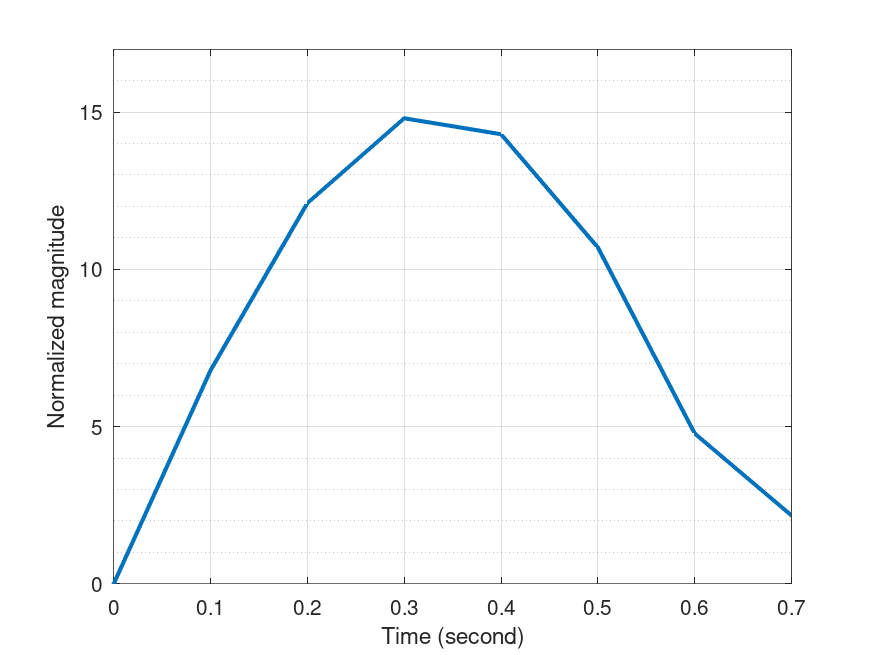
\includegraphics[width=0.5\linewidth]{../../../soal/kuis/soal1_kuis2}
	\end{figure}
\end{frame}

\begin{frame}[t]{Soal 1}
	\begin{figure}
		\centering
		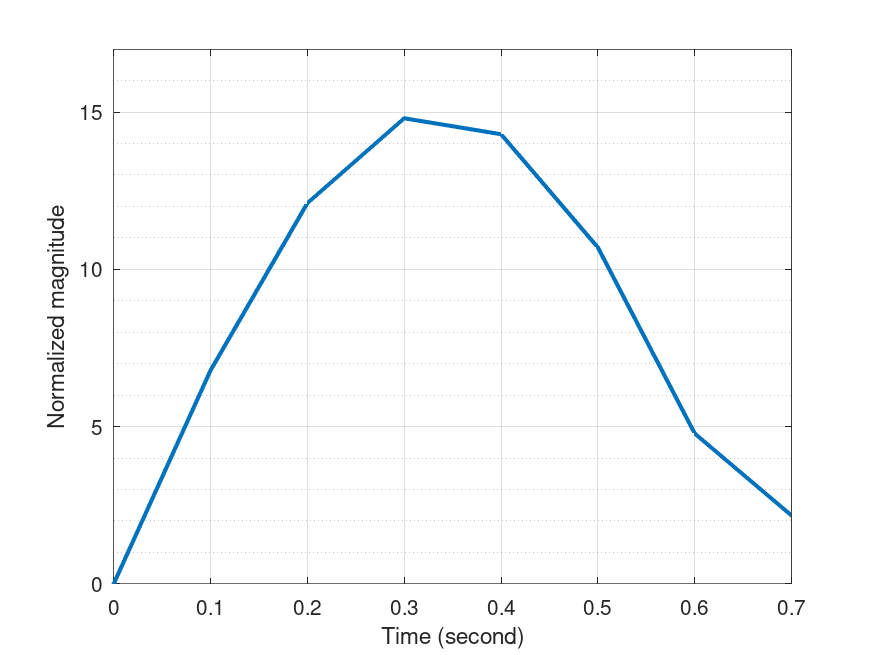
\includegraphics[width=0.5\linewidth]{../../../soal/kuis/soal1_kuis2}
	\end{figure}
\end{frame}

\begin{frame}[t]{Soal 1}

\end{frame}


\section{Soal 2}

\begin{frame}[t]{Soal 2}
	\begin{itemize}
		\item Jika diketahui data analog sebagai berikut, tentukan sinyal digitalnya dengan menggunakan teknik DM.
	\end{itemize}
	\begin{figure}
		\centering
		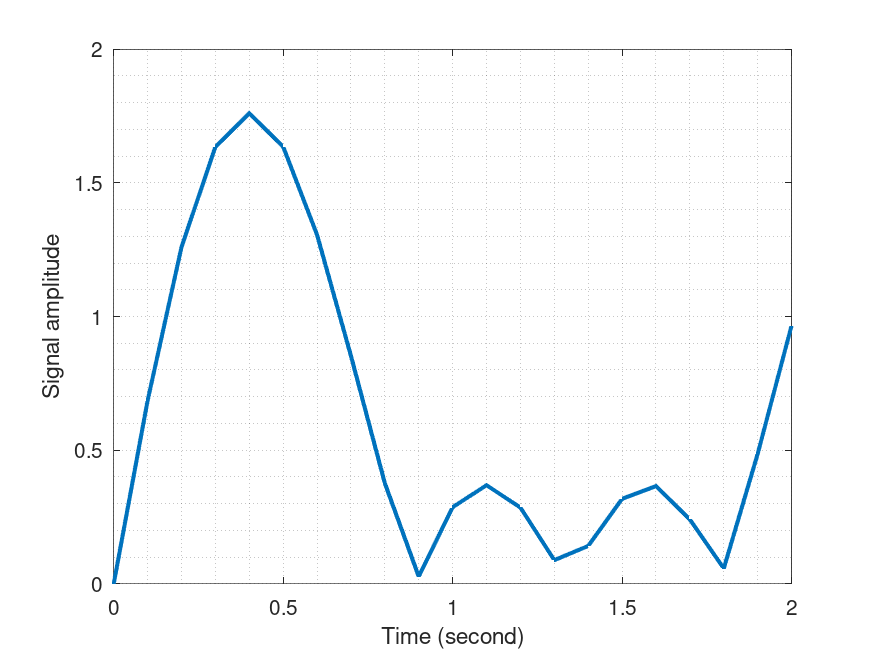
\includegraphics[width=0.5\linewidth]{../../../soal/kuis/soal2_kuis2}
	\end{figure}
\end{frame}

\begin{frame}[t]{Soal 2}
	\begin{figure}
		\centering
		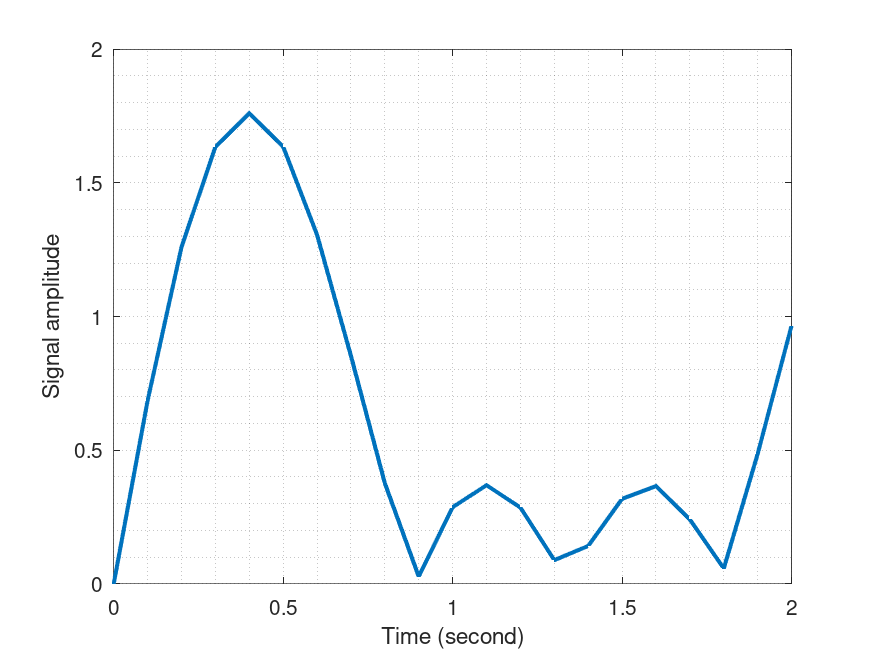
\includegraphics[height=0.9\textheight]{../../../soal/kuis/soal2_kuis2}
	\end{figure}
\end{frame}

\begin{frame}[t]{Soal 2}
	
\end{frame}


\section{Soal 3}

\begin{frame}[t]{Soal 3}
	\begin{itemize}
		\item Jika data yang dikirim adalah sebagai berikut:\\
		
		\begin{tabular}{cccccccccccccccc}
			1 & 1 & 0 & 1 & 1 & 0 & 1 & 0 & 1 & 0 & 1 & 0 & 1 & 1 & 0 & 0 \\
		\end{tabular}
	
		\item Sedangkan yang diterima adalah sebagai berikut: \\
		
		\begin{tabular}{cccccccccccccccc}
			1 & 1 & 0 & 1 & 0 & 0 & 1 & 0 & 1 & 1 & 0 & 1 & 1 & 1 & 1 & 0 \\
		\end{tabular}
		\item Tentukan berapa panjang dari burst error-nya.
	\end{itemize}
\end{frame}

\begin{frame}[t]{Soal 3}
	\begin{itemize}
		\item Data yang dikirim:\\
		
		\begin{tabular}{cccccccccccccccc}
			1 & 1 & 0 & 1 & 1 & 0 & 1 & 0 & 1 & 0 & 1 & 0 & 1 & 1 & 0 & 0 \\
		\end{tabular}
		
		\item Data yang diterima: \\
		
		\begin{tabular}{cccccccccccccccc}
			1 & 1 & 0 & 1 & 0 & 0 & 1 & 0 & 1 & 1 & 0 & 1 & 1 & 1 & 1 & 0 \\
		\end{tabular}
	
	\end{itemize}
\end{frame}

\begin{frame}[t]{Soal 3}
	
\end{frame}

\section{Soal 4}

\begin{frame}[t]{Soal 4}
	\begin{itemize}
		\item Jika digunakan teknik 2D even parity, buktikan apakah terjadi error pada data berikut ini? Dan berapakah nilai seharusnya?
	\end{itemize}

	\begin{figure}
		\centering
		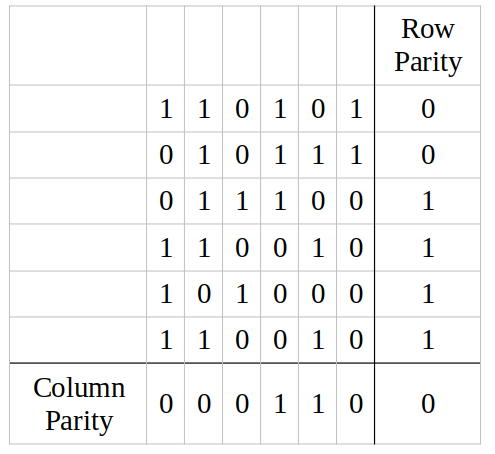
\includegraphics[width=0.4\linewidth]{../../../soal/kuis/soal4_kuis2}
	\end{figure}
\end{frame}

\begin{frame}[t]{Soal 4}
	\begin{figure}
		\centering
		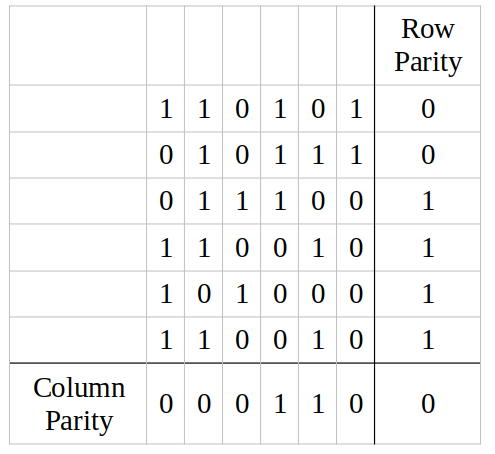
\includegraphics[width=0.5\linewidth]{../../../soal/kuis/soal4_kuis2}
	\end{figure}
\end{frame}

\begin{frame}[t]{Soal 4}
	
\end{frame}

\section{Soal 5}

\begin{frame}[t]{Soal 5}
	\begin{itemize}
		\item Diketahui data stream yang diterima adalah sebagai berikut.
		
		\begin{figure}
			\centering
			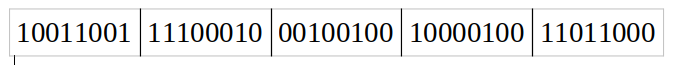
\includegraphics[width=0.9\linewidth]{../../../soal/kuis/soal5_kuis2}
		\end{figure}
		
		\item Dengan menggunakan internet checksum, buktikan bahwa data tersebut terdapat error.
	\end{itemize}
\end{frame}

\begin{frame}[t]{Soal 5}
	\begin{itemize}
		\item Data stream yang diterima:
		\begin{figure}
			\centering
			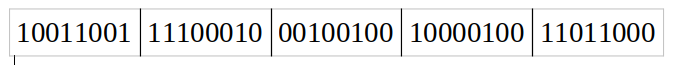
\includegraphics[width=0.9\linewidth]{../../../soal/kuis/soal5_kuis2}
		\end{figure}
	\end{itemize}
\end{frame}

\begin{frame}[t]{Soal 5}
	
\end{frame}


\section{Soal 6}

\begin{frame}[t]{Soal 6}
	\begin{itemize}
		\item Dengan menggunakan teknik CRC dengan CRC generatornya adalah $ x^3 + 1 $, buktikan apakah data stream berikut ini diterima atau tidak.
		
		\begin{figure}
			\centering
			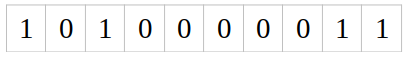
\includegraphics[width=0.4\linewidth]{../../../soal/kuis/soal6_kuis2}
		\end{figure}

	\end{itemize}
\end{frame}

\begin{frame}[t]{Soal 6}

\end{frame}


\end{document}

